\documentclass{article}
\usepackage{graphicx} % Required for inserting images
\usepackage{amsmath}
\usepackage{amsthm}
\usepackage{amssymb}
\usepackage{float}
\usepackage{booktabs}
\usepackage[margin=1in]{geometry}
\newcommand{\todo}[1]{\textbf{[#1]}}

\usepackage[hidelinks]{hyperref}
\usepackage{parskip}


\title{Bail(ey)ing Out: An Agent-Based Model of Evacuation Under Crowd Management}
\author{Jason Zhang, Hendry Xu, Lexiang Sun}
\date{November 2026}

\begin{document}

\maketitle
\begin{center}
\textbf{Abstract}
\end{center}

Bailey Hall seats 1,329 people, and the University's target is to empty it within 180 seconds of an emergency being declared. We build a stochastic agent-based cellular-automaton model of the hall: a to-scale graph of both levels with every seat, aisle, door and staircase, on which each audience member responds to the alarm after a seat-dependent, log-normally distributed delay, walks at an individual speed, weighs the shortest route against the movement of the crowd, and chooses among the exits they know about. Crowd Managers redirect people near their posts, exits can be blocked without warning, temporary barriers can partition the corridor, and directional LED strips can bias movement.

No scenario we simulated meets the 180-second target. A full concert audience guided by six Crowd Managers takes 220\,s on average, students who know every exit take 227\,s, and an ordinary departure through the front doors takes 254\,s. The binding constraint is the pair of 4-ft portico doors, which are the nearest exits for anyone leaving the loge by a side door and end up carrying more than half of the audience; because of them, students' knowledge of the building buys them nothing. An unexpected closure of two front doors costs almost nothing, while closing a portico door adds about 16\,s. Optimizing the six Crowd Managers' posts saves about 7\%, with no benefit from a seventh or eighth. Corridor barriers do not shorten a typical concert evacuation but remove its worst cases, and they slow students down. Directional LED strips up the two centre aisles of the orchestra, which pull people away from the portico doors toward the under-used front doors, save about 30\,s, twice what the managers achieve, for a one-time cost comparable to one extra manager over a season or two. Together, optimized managers and LED strips should bring a concert evacuation close to 180 seconds.

\newpage
\section*{Executive Summary}
\addcontentsline{toc}{section}{Executive Summary}

{\small
\setlength{\parskip}{4pt}
\noindent\textbf{To:} Mr.\ Timothy Ryan, University Fire Marshal and Director of Fire Protection and Emergency Services\\
\textbf{From:} Jason Zhang, Hendry Xu, Lexiang Sun\\
\textbf{Re:} Evacuation of Bailey Hall: what limits it, and what would help

\medskip
\noindent Dear Mr.\ Ryan,

We simulated a full Bailey Hall (all 1,329 seats, both levels) in which every person reacts to the alarm, chooses a door and walks out, influenced by the crowd, by Crowd Managers and by what they know of the building. Each scenario was simulated 24 times.

\textbf{What we found.}\vspace{-4pt}
\begin{itemize}
    \item \textbf{The 180-second target was not met in any scenario.} A concert audience with six Crowd Managers is out in about 220\,s on average; a lecture of students who know every exit, in about 227\,s; an ordinary end-of-concert departure through the front doors, in about 254\,s.
    \item \textbf{The two portico doors are the bottleneck.} The 4-ft doors on either side of the corridor are the nearest exit for everyone leaving the loge by a side door, so each takes roughly 400 people and is always the last to clear, while the five front doors finish well before. That is why students, who know every exit, are no faster: each heads for their own nearest door. Reaction matters too (half an audience is not moving 51\,s after an alarm), but most people are ready long before their turn at a portico door.
    \item \textbf{The current exits are robust to a blocked front door.} With the two central front doors blocked, the time barely changes. A blocked portico door adds about 16\,s; managers who know of it send people to the stage escape routes.
    \item \textbf{Crowd Managers help, but the sixth is the last one that pays.} Well-placed posts save about 7\%; a seventh or eighth manager made no measurable difference.
    \item \textbf{Directional LED strips help the most.} Two strips running up the centre aisles of the orchestra, through the aisle doors and on to the front doors, draw people away from the overloaded portico doors and saved about 30\,s in our simulations, twice the effect of optimizing the managers. Combined with optimized managers, we estimate a concert evacuation of about 180\,s.
    \item \textbf{Temporary corridor barriers are a modest, concert-only measure.} Barriers across the corridor between each portico door and the foyer did not shorten a typical concert evacuation, but they prevented the occasional jams at the portico doors (worst case 234\,s instead of 276\,s with managers). They slowed students down, so they should be used for concerts only.
\end{itemize}

\textbf{Our recommendations}, in order of value for money:
\begin{enumerate}
    \item \textbf{Install directional LED strips} along the two centre aisles to the front doors (about 53\,m, roughly \$4,000--\$7,500 including battery backup), \textbf{wired to the fire alarm panel} so that a strip leading to a blocked door can be switched off. This costs about the same as one extra Crowd Manager for one or two seasons, and works at every event.
    \item \textbf{Re-post the six Crowd Managers} to the mid cross aisles and side corridors on the first floor and the south ends of the balcony, and \textbf{brief them on the portico doors}: when the portico queues grow, the most valuable instruction is to send people to the front doors or the stage escape routes.
    \item \textbf{Set up the corridor barriers for concerts} (not lectures): they cost under \$1,500, are reusable, and make the evacuation more predictable.
    \item \textbf{Announce the evacuation immediately} from the stage and by every manager, to cut the reaction delay; it costs nothing. \textbf{Do not hire managers beyond the legal six} for speed; the money is better spent on LEDs.
\end{enumerate}

We are sanguine that, with these changes, a well-rehearsed choreography of announcements, managers and lights can bring the evacuation much closer to the target, but we cannot honestly promise 180 seconds: our model's door flows are, if anything, optimistic. Above all, any plan should keep its legibility: one strip, one door, one instruction per area, so that it still works when it is executed by frightened people.

\medskip
\noindent Sincerely,\\
Jason Zhang, Hendry Xu, Lexiang Sun
}

\newpage
\tableofcontents

\newpage
\section{Introduction}
\subsection{Background information}
\begin{figure}[H]
    \centering
    \includegraphics[width=0.5\linewidth]{bailey hall.jpeg}
    \caption{Bailey Hall}
    \label{fig:bailey}
\end{figure}
From concerts to comedy shows, Bailey Hall hosts a variety of events for Cornellians. With an auditorium capacity of 1,329 people, an important consideration when operating a venue of this size is whether people can exit quickly and safely during an emergency. This process can be complicated as people may be influenced by those around them, and have differing senses of urgency and reaction speeds. To aid in an orderly evacuation, New York State law requires at least one Crowd Manager per 250 attendees, so at least six Crowd Managers must be present during a full-capacity, non-academic event. To facilitate the work of Crowd Managers and ensure the safety of the attendees, the university needs a plan for where Crowd Managers are positioned and whether minor modifications to the building can help it meet its 180-second evacuation target.

\subsection{Problem Statement}
We are asked to analyze the dynamics of large-scale egress and evacuation from Bailey Hall. Of the questions posed, we address the following:
\begin{enumerate}
    \item[(Q1)] How long does it take a full concert audience to leave after a concert, under normal, calm circumstances?
    \item[(Q2)] How long does an emergency evacuation of the same audience take when guided by six Crowd Managers, and how does that change when an exit is unexpectedly obstructed?
    \item[(Q3)] How does this compare with an evacuation of 1,329 students from a lecture, where there are no Crowd Managers but everyone knows every exit?
    \item[(Q4)] Can egress be made faster, safely, by (a) temporary barriers in the corridor that restrict which exterior doors people from each auditorium door can reach, or (b) directional LED strips that guide different parts of the audience to specific exits? For concerts these measures help the six Crowd Managers rather than replace them.
    \item[(Q5)] Are these measures cost-effective compared with hiring more Crowd Managers?
\end{enumerate}
Following the organizers' advice, Questions (2), (3) and (4) are our main focus; (1) and (5) are shorter extensions.

\subsection{Literature Review}
Building evacuation models are important and widely studied;
\cite{nist2010} offers a comprehensive review of the types of models that already exist. Different models can be implemented based on the problem at hand, and they can be categorized based on structure, perspective of the occupant, behavior, movement, and various other features.

In general, these models differ in how they represent pedestrian movement. Some model evacuation as a flow of people through a corridor, essentially tracking the crowd as a single macroscopic quantity. Others follow individual occupants as they move through a discretized space. For the latter, \cite{burstedde2001} proposes a standard cellular automaton model, where pedestrians move between cells on a two-dimensional grid. Each cell can hold at most one pedestrian, and their movement probabilities are governed by floor fields. \cite{kirchner2002} extend this with a dynamic floor field that lets pedestrians follow the trails of others, a simple form of herding.

We take the individual-based approach. A flow model would require us to conjecture about the emergent properties of the crowd, such as how quickly a bottleneck drains or how congestion builds near a door, before we have simulated anything. In an agent-based model, those properties arise on their own from the characteristics of the individuals, which we have a much better intuitive and experience-based understanding of. Most of us have been part of a crowd leaving a venue, so we can reason about why one person picks a certain door, follows the people ahead of them, or waits. This approach also gives us a more detailed picture of pedestrian interactions and congestion, and lets us build in behavioral rules for individual decisions.

A study on evacuation dynamics of the Marlowe Theatre \cite{galea2017} found that audience members' response times to an alarm approximately followed a log-normal distribution and were influenced by their seating locations. In particular, average response times generally increased with both the distance of an individual's seat from the nearest aisle and the distance of their seating row from an exit. Building on these findings, our model extends the basic cellular automaton framework by incorporating log-normally distributed individual response times that depend on seating location.

\subsection{Our Approach}
Our proposed model follows the fine-network approach described by \cite{burstedde2001}, in which the building is discretized into individual cells and pedestrians move between available cells. We incorporate behavioral elements informed by \cite{galea2017}, assigning a response time to each pedestrian based on their seating location. Once this time has elapsed, the pedestrian is ready to evacuate and enter the movement phase.

Each cell can hold at most one pedestrian, so physical obstructions and congestion arise naturally. We also differentiate moving speeds between seating rows, stairs and open corridors. At each time step, the pedestrian selects their next movement probabilistically, based on (1) how much closer the move brings them to their current target, (2) the recent movement directions of nearby pedestrians, weighted by proximity, (3) their own independence, which sets how much they weigh their target against the crowd, and (4) the pull of any visible LED strips, scaled by how much they trust them. Only unoccupied neighboring nodes are considered (walls, barriers and closed exits are not walkable). Their walking speed then determines whether they can afford to make their chosen move on that step. Exit selection can also be influenced by Crowd Managers and unexpected blockages.

Using this framework, we simulate different evacuation scenarios and evaluate how different crowd-managing strategies affect total evacuation time. We then search over Crowd Manager posts and LED strip layouts with a greedy simulation-based optimization.

\subsection{Model Assumptions}

\textbf{Population and Behavior}
\begin{itemize}
    \item The hall is full: all 1,329 seats (527 orchestra, 486 loge, 316 balcony) are occupied.
    \item Each person acts on individual motivation alone, and no groups or families wait or go back for one another. We justify this by assuming that adult groups trust each other enough to let one another act independently, and that at-risk people such as children or the elderly set the speed of their group, so the group can be treated as a single agent with a slower speed.
    \item Everyone receives the emergency alarm at the same time, though they may take different amounts of time to start evacuating. The emergency occurs once everyone is seated.
    \item As previous literature shows, people generally respond calmly \cite{simeHUMANBEHAVIOURFIRES}. No mass panic occurs.
    \item Response times do not depend on the stage of the event (before the show, just started, mid-performance, or ending).
\end{itemize}

\textbf{Information and Decision-Making}
\begin{itemize}
    \item An exit is ``visible'' if it lies within 15\,m of walking cost. We do not model line of sight.
    \item People notice a closed exit only when within 4\,m of walking distance, and do not communicate this to others.
    \item People re-evaluate their target every 30 time steps (about 11\,s), choosing stochastically with a preference for nearer options.
    \item Anyone who reaches an open exit leaves through it, even if they were aiming for a different exit.
\end{itemize}

\textbf{Exit Knowledge and Navigation}
\begin{itemize}
    \item Non-student, non-performer audience members are aware only of:
    \begin{itemize}
        \item exits they can see,
        \item exits indicated to them by a Crowd Manager, and
        \item the main door through which they entered.
    \end{itemize}
    \item Every member of the concert audience begins with the same goal: to leave the building through the main exits. From their seat, each person heads for the closest door leading from the auditorium into the halls outside.
    \item Each person can always correctly determine which of the currently visible exits is closest to them.
    \item During evacuations of the general public, no one is familiar with the entire floor plan of Bailey Hall. Students who know the building are most likely among the performers on stage, so they are not positioned to guide audience members toward exits. During student evacuations of lectures, all students are assumed to be familiar with the layout of Bailey Hall.
    \item The two stage escape routes (SW and SE) are unknown to the concert audience unless a Crowd Manager sends them there.
    \item All individuals avoid using elevators during the emergency.
    \item The service, performer and ground-level spaces are ignored, as the problem statement allows.
\end{itemize}

\textbf{Crowd Managers, Barriers and LED Guidance}
\begin{itemize}
    \item Crowd Managers are stationary, active from the moment of the alarm, and know about all exit closures from the start. They do not occupy floor space.
    \item Crowd Managers redirect people within their radius at a rate that grows with proximity. Redirected people follow the instruction without further re-evaluation of their exit. Managers execute their instructions without error.
    \item Temporary barriers are placed before the event, are visible to everyone, and are respected: nobody climbs over or moves them.
    \item LED strips are passive. They influence how a person moves but never assign or change their target door or exit. Each strip is fixed and does not sense or respond to crowding, closures, or the actions of Crowd Managers, so a strip may point toward a closed exit.
    \item The influence of a strip decays exponentially with walking distance and vanishes beyond 15\,m. It is also scaled by how much the individual trusts the strips, and that trust falls each time the strips lead someone to a closed exit.
\end{itemize}


\newpage
\section{Model}
In this section we present our model for the egress of a full audience from Bailey Hall, both in an emergency guided by Crowd Managers and in the other scenarios of Section~\ref{sec:design}. We model egress as a stochastic, discrete-time, agent-based cellular automaton.

Each person is an agent. Open floor is tiled by a grid of $0.5\,\text{m}\times 0.5\,\text{m}$ cells, and seats are separate nodes (Section~\ref{sec:building}). Every node holds at most one agent. In each time step, an agent may move to an unoccupied neighboring node, that is, one that shares an edge or a corner with its current cell. If none is available, it stays where it is. Agents move one at a time in a random order (Section~\ref{sec:order}), so two agents can never enter the same node.

\subsection{Building representation}
\label{sec:building}
\begin{figure}[H]
    \centering
    \includegraphics[width=1.0\linewidth]{grid_hybrid.png}
    \caption{Discrete grid model of Bailey Hall: the first floor (left) and the balcony (right).}
    \label{fig:grid}
\end{figure}

We built a to-scale geometric model of Bailey Hall from the evacuation plans and seating charts supplied with the problem. We calibrated the scale of each drawing from dimensioned features such as the 27\,ft centre block and the row pitch, and expect positions to be accurate to about $\pm 2\%$. The model has two levels: the first floor (orchestra, loge, corridor, vestibule and foyer) and the balcony. Exits from the building are labelled as in Figure~\ref{fig:grid}:
\begin{itemize}
    \item F1--F5: the five front doors of the foyer (5.5\,ft each), the usual way out;
    \item PW, PE: the portico doors on the west and east sides of the corridor (4\,ft each);
    \item SW, SE: the stage escape routes on either side of the stage;
    \item BW, BE: the stage-side balcony doors, which lead down a staircase directly outside.
\end{itemize}
The auditorium itself has five doors on the first floor (the two aisle doors, the two side-aisle doors and the centre door, all in the back wall of the loge) and four on the balcony (the two doors to the main balcony staircases, which land beside the foyer, and BW/BE). The problem statement mentions nine first-floor doors; the drawings show five openings, four of them pairs of leaves, so we model those as single 5\,ft openings and the centre door as 6\,ft.

We represent the hall using a hybrid discrete spatial model, shown in Figure~\ref{fig:grid}. Open areas, such as corridors, aisles, and foyers, are discretized into a $0.5\,\text{m} \times 0.5\,\text{m}$ lattice. We chose this cell size because it is approximately the width of the space occupied by one standing adult (roughly shoulder width).

Seating areas are represented differently. We do not subdivide each row into regular $0.5\,\text{m}$ cells because people must start at their actual seats but the seats are not clean multiples of the grid size, so matching the true seat geometry with a regular lattice would be difficult.

Instead, each seat is represented by two nodes: a \textbf{seat node}, where the person sits, and a \textbf{standing node}, the walkable space in front of the seat that the person occupies once they are up and moving. A one-way edge connects each seat node to its standing node, so a person can leave their seat but never return to it.

The building is therefore represented by a directed graph $G=(V,E)$, where
\[
V = V_{\text{walk}} \cup V_{\text{seat}} \cup V_{\text{stand}} \cup V_{\text{stair}}.
\]
Here, $V_{\text{walk}}$ is the set of walkable lattice cells, $V_{\text{seat}}$ the set of seat nodes, $V_{\text{stand}}$ the set of standing nodes, and $V_{\text{stair}}$ the set of intermediate stair nodes. An edge $(u,v)\in E$ is included whenever a pedestrian may move directly from $u$ to $v$. Edges are directed because some connections, such as seat to standing node and each staircase lane, work in only one direction. The final graph has 2,428 lattice cells, 1,329 seat nodes, 1,329 standing nodes, 48 stair nodes and 21,651 edges.

Walkway cells are connected to their eight neighboring walkway cells, without cutting corners past a wall. Standing nodes are connected to neighboring standing nodes in the same row and, at the ends of each row, to the nearest aisle cell, so a person can walk along the row to the aisle. Walls, impassable regions, and placed temporary barriers are excluded from the graph. Exit doors are represented as special walkable nodes.

Each main balcony staircase is represented by two parallel, one-way chains of nodes connecting the balcony to the first-floor landing beside the foyer, so people move along it node by node. This lets several pedestrians be on a staircase at once while preventing any two from sharing a position. The stage-side balcony stairs are not in the graph; a person who leaves through BW or BE is out of the auditorium at the door, and we add the time they need to walk down that 32\,ft staircase at stair speed.

\textbf{Edge costs.} Every edge has a length $L(e)$ in meters and a cost. The cost is the length multiplied by a factor for the node being entered: 1 for floor, doors and standing nodes, 2 for stairs and 2.5 for seat nodes. The factor expresses that people move more slowly, and choose routes accordingly, on stairs and between rows of seats. All the route costs $D$ below are computed with this weighted cost, so a cost of 15 ``meters'' on a stair is only 7.5\,m of actual stair.

At the start of the simulation, each seat node contains exactly one agent and all other nodes are empty.


\subsection{Response Time}
\label{sec:response}

We denote $T_i$ to be the response time of pedestrian $i$
before accounting for social influence.
Note that this represents the time between the sounding of
the alarm and when the pedestrian is ready to start moving,
not necessarily when their physical movement begins.
A pedestrian may be ready to move but remain blocked by
an adjacent occupant.

To assign response times that follow the findings of
\cite{galea2017}, suppose there are $N$ audience members.
We independently sample their response times (in seconds) from the
log-normal distribution determined by the study:

\begin{equation}
    S_1, \ldots, S_N \overset{\mathrm{i.i.d.}}{\sim}
    \operatorname{Lognormal}(3.93, 0.44^2),
\end{equation}
which has a median of 51\,s and a mean of 56\,s.
We then sort the sampled response times in ascending order:

\[
    S_{(1)} \leq S_{(2)} \leq \cdots \leq S_{(N)}.
\]

Next, for each seat $i$, we define:
\begin{itemize}
    \item $d_i^{\mathrm{aisle}}$: the number of seats
    separating seat $i$ from the nearer end of its row.

    \item $d_i^{\mathrm{row}}$: the number of rows
    separating seat $i$ from the nearer end of its seating section. (In the two upper side boxes on the first floor the only aisle is below the box, so there $d_i^{\mathrm{row}}$ counts from the bottom.)
\end{itemize}

We then order the seats primarily by increasing
$d_i^{\mathrm{aisle}}$, followed by increasing
$d_i^{\mathrm{row}}$, breaking ties randomly.
The sorted response times are assigned to the seats
in this order, with shorter response times assigned
to seats appearing earlier in the ordering.
We denote the initially assigned response time of
pedestrian $i$ by $T_i^{(0)}$.

However, this relationship may not hold for every individual.
To account for individual variation, we randomly redistribute
20\% of the assigned response times, following the methodology
proposed by \cite{galea2017}.

To do this, we randomly select a subset $A$ containing
20\% of the audience and shuffle their
assigned response times, leaving the remaining 80\% unchanged.

Let $\pi$ be a uniformly random permutation of $A$.
The response time of pedestrian $i$ after redistribution
is given by

\begin{equation}
    T_i =
    \begin{cases}
        T_{\pi(i)}^{(0)}, & i \in A,\\
        T_i^{(0)}, & i \notin A.
    \end{cases}
    \label{eq:randomized_response}
\end{equation}

Finally, we incorporate social influence, since pedestrians
may respond earlier upon observing others beginning to
evacuate. We assume that each pedestrian can only observe
the movements of their immediate neighbours in the same
seating row. Once a neighbouring pedestrian begins moving,
the observing pedestrian becomes ready after an additional
delay of $\tau = 5$ seconds, unless their original response
time occurs sooner.

Let $t_i^{\mathrm{observe}}$ denote the first time pedestrian
$i$ observes an immediate neighbour beginning to move.
The effective response time is then

\begin{equation}
    \widehat{T}_i =
    \min\left(T_i,\,
    t_i^{\mathrm{observe}}+\tau\right).
    \label{eq:social_response}
\end{equation}

If neither neighbour begins moving before $T_i$, the
original response time is retained. This influence can
propagate along a row, but can only shorten,
never increase, response times.

\subsection{Walking Speed and Movement}
\label{sec:movement}

Once an agent is ready to evacuate, its motion is governed by three components: how far it is allowed to walk in a given time step (the movement budget), which neighboring node it prefers (the movement rule), and in what order agents are resolved when they compete for space. We describe each below.

\subsubsection{Time Step and Movement Budget}
\label{sec:budget}

We use a cell size of $\Delta = 0.5$\,m and a free-flow walking speed of
$v_{\max} = 1.4$\,m/s for an unimpeded pedestrian. This is consistent with the
empirical literature, which reports a mean free-flow speed of about
$1.34$\,m/s with a standard deviation of roughly $0.26$\,m/s
\cite{weidmann1993,helbing1995}, and averages near $1.4$\,m/s in European
studies \cite{daamen2007}. One time step corresponds to the time needed to
cross one cell at this speed,
\begin{equation}
    \Delta t = \frac{\Delta}{v_{\max}} \approx 0.36\ \text{s}.
\end{equation}
The simulation therefore advances in uniform steps, but people do not all walk
at the same speed. Because our simulation only allows agents to move 0 or 1
cells per step, we introduce a \textbf{movement budget} to handle different
speeds.

We treat $v_{\max}$ as an upper limit rather than a typical speed. Each agent $i$ is assigned a speed fraction $s_i \in [0.3, 1]$, drawn once at the start of the simulation from a normal distribution clipped to that interval,
\begin{equation}
    s_i = \operatorname{clip}\!\big(\mathcal{N}(0.8,\,0.15^2),\ 0.3,\ 1\big),
\end{equation}
so that agent $i$ has a preferred walking speed of $s_i \cdot v_{\max}$, ranging from $0.42$ to $1.4$\,m/s and averaging about $1.1$\,m/s. This is somewhat below the free-flow mean reported in the literature. We choose it because free-flow measurements describe unobstructed walking on open, level ground, whereas evacuees here move through curved seating rows, narrow aisles and stairs, often carrying belongings in an unfamiliar building, and the audience includes children, older adults and others who walk slowly \cite{bohannon1997}. Egress design guidance likewise uses unimpeded speeds below the free-flow mean. The lower speeds also make our evacuation times conservative estimates.

Each agent also carries a budget $B_i$, measured in meters and initially $0$. At the start of every time step the budget grows by the distance the agent can cover in one step at its own speed,
\begin{equation}
    B_i \leftarrow B_i + s_i\,\Delta .
\end{equation}
When an agent has chosen an edge $e$ of length $L(e)$ (Section~\ref{sec:selection}), it may traverse the edge only if it can afford it,
\begin{equation}
    B_i \ge L(e), \qquad \text{in which case} \qquad B_i \leftarrow B_i - L(e).
\end{equation}
Otherwise the agent stays where it is for this step and keeps its budget, which carries over to later steps. An agent makes at most one move per time step.

\subsubsection{Movement selection}
\label{sec:selection}

Let $D(x)$ be the cost from node $x$ to the agent's current target (an auditorium door or a building exit), computed with Dijkstra's algorithm as the shortest-path cost on the graph. Walls are not part of the graph, and barriers are treated as blocked. The candidate moves are the neighboring nodes $v$ that are unoccupied and from which the target is reachable. Once an agent has left the seating area it may not re-enter a seat node. For each candidate, the agent computes the cost gained,
\begin{equation}
g(v) = D(u) - D(v),
\end{equation}
which is positive when the move brings the agent closer to their target.

\textbf{Agents are also influenced by the movement of people around them.} Each agent remembers the compass direction of its last move (the eight directions are numbered $j = 0, \dots, 7$). For agent $i$ at $u$, every other agent $k$ standing within $r = 2$\,m of $u$ (on the same level) is a neighbor and receives the weight $w_k = e^{-d_k}$, where $d_k$ is its distance from $u$ in meters. Let $W_j$ be the total weight of neighbors whose last move was in direction $j$, and let $W$ be the total weight of all neighbors. The crowd's preference for direction $j$ is
\begin{equation}
h_j = \frac{W_j}{W}.
\end{equation}
Neighbors that have not yet moved count in $W$ but not in any $W_j$. If there are no neighbors, $h_j = 0$.

Each agent has an \emph{independence} $I_i \ge 1$, drawn once from a normal distribution (Section~\ref{sec:profiles}), which measures how much they care about the shortest route as opposed to following the crowd. If the move from $u$ to $v$ points in direction $j(v)$, the agent assigns it the score
\begin{equation}
z_i(v) = 3 I_i\, g(v) + \frac{2H}{I_i^{2}}\, h_{j(v)} + \ell_i(u,v),
\label{eq:score}
\end{equation}
where $H = 2$ is the herding strength and $\ell_i(u,v)$ is the LED term, which is zero unless the agent can see an LED strip (Section~\ref{sec:led}). It then chooses $v$ among the candidates with probability
\begin{equation}
P(v) = \frac{e^{z_i(v)}}{\sum_{v'} e^{z_i(v')}} .
\end{equation}
The first term is the selfish pull toward the target and grows linearly with independence. The second is the herd pull and falls off with $I_i^2$, so a more independent agent is influenced by the crowd less.

\subsubsection{Update order and conflicts}
\label{sec:order}

In each time step, agents are processed sequentially in a random order that is redrawn every time step. The occupancy of each node is updated immediately after each move. An agent therefore always sees the current occupancy, and two agents can never enter the same node. When several agents want the same cell, whichever is processed first gets it, and the random ordering ensures no agent has a systematic advantage. An agent stays in place for the step if it has no free neighboring node, or if its budget $B_i$ is smaller than the length $L$ of the edge it chose (Section~\ref{sec:budget}).

\subsection{Targets and Re-evaluation}
\label{sec:targets}

Because the auditorium is enclosed by the corridor, every agent must leave the auditorium before it can leave the building. We therefore split each agent's evacuation into two stages, each with its own target. An agent first heads for a door out of the auditorium. Once it reaches any door it knows to be usable, it switches its target to a building exit. When it reaches a building exit, it leaves the simulation and its node is freed. Students whose nearest exit is not behind an auditorium door (the stage escape routes) skip the first stage.

Agents do not commit permanently to their initial targets. Every $T = 30$ time steps (staggered across agents so that agents re-decide in batches), each agent picks a new target $k$ from its available options with probability
\begin{equation}
P(k) = \frac{e^{-\beta\,\left(D_k(u) - D_{\min}(u)\right)}}{\sum_{k' \in \mathcal{K}} e^{-\beta\,\left(D_{k'}(u) - D_{\min}(u)\right)}},
\end{equation}
where $\mathcal{K}$ is the set of options currently visible to the agent, $D_k(u)$ is the cost from the agent's current node $u$ to option $k$, $D_{\min}(u) = \min_{k' \in \mathcal{K}} D_{k'}(u)$ is the smallest such cost, and $\beta = 1$ controls how strongly the nearest option is favored. An option is \emph{visible} only if its cost from $u$ is at most the view range $R = 15$, with the exception that an agent always keeps its current target (door or exit) among its options if it is still reachable. Without this exception, a person could flip between two doors indefinitely as each drops in and out of view. If no option is visible, the agent keeps its current target. In addition to the periodic re-evaluation, an agent chooses its exit by the same rule the moment it steps out of the auditorium: someone entering the corridor looks around and sees the doors and barriers in front of them, rather than walking on toward a front door for up to another 11\,s. The set of options depends on what the agent knows, which is the main difference between the audience types (Section~\ref{sec:profiles}).

This allows agents to reconsider their routes as they move and discover alternative exits, while maintaining a preference for shorter paths.

\subsection{Audience Types: Concert Attendees versus Students}
\label{sec:profiles}

We simulate two kinds of audience that differ in two ways: how well they know the building, and how strongly they follow the crowd. Both use the same movement rule (Equation~\ref{eq:score}); only the parameters and the options they consider differ (Table~\ref{tab:profiles}).

\begin{table}[H]
    \centering
    \begin{tabular}{lcc}
        \toprule
         & \textbf{Concert} & \textbf{Students} \\
        \midrule
        Knows all exits of the building & No & Yes \\
        Independence $I_i$ (mean, s.d.) & $3.0,\ 1.0$ & $4.5,\ 1.0$ \\
        Independence minimum & $1$ & $1$ \\
        Speed fraction $s_i$ (mean, s.d.) & $0.8,\ 0.15$ & $0.8,\ 0.15$ \\
        Crowd Managers present & Yes (6) & No \\
        \bottomrule
    \end{tabular}
    \caption{Parameters of the two audience profiles. The independence $I_i$ is clipped below at $1$, and the speed fraction is clipped to $[0.3,1]$.}
    \label{tab:profiles}
\end{table}

\textbf{Concert attendees (general public).} Following our assumptions, general-public attendees do not know the floor plan, so their choices are limited to the doors and entrances they are aware of. Their initial plan is to leave through the main entrances: from their seat each person picks the cheapest of the nine auditorium doors, and the cheapest of the five main entrances $F_1,\dots,F_5$ as their building exit. At re-evaluation (Section~\ref{sec:targets}), the options in $\mathcal{K}$ depend on the stage. While heading to a door, an attendee chooses among the auditorium doors by the cost to the door alone. Once out of the auditorium, an attendee chooses among the five main entrances and the two portico doors PW and PE, restricted to those within view range, so an attendee who notices a portico door on the way out can switch to it without being told. No other exit enters their own choices. Two outside influences can override these choices: a Crowd Manager (Section~\ref{sec:managers}) and LED strips (Section~\ref{sec:led}). Their mean independence is lower ($3.0$), so they are more strongly drawn by the movements of the people around them.

\textbf{Students.} In the lecture setting all students are assumed to know the layout of Bailey Hall. From their seat, a student identifies the cheapest exit of the \textbf{whole building}, $e^\ast(i)=\arg\min_{k} D_k(\text{seat}_i)$, and then picks the auditorium door lying on the cheapest route to it,
\begin{equation}
    \text{door}^\ast(i) = \arg\min_q \big[ D_q(\text{seat}_i) + D_{q \to e^\ast}\big],
\end{equation}
where $D_q$ is the cost to door $q$ and $D_{q\to e^\ast}$ the cost from that door to the exit. At re-evaluation, a student heading to a door scores each door by the total cost through it to the current exit target (visibility is still judged by the distance to the door itself), and a student heading to an exit chooses among \emph{all} open exits of the building. Their mean independence is higher ($4.5$), so they rely less on the crowd and more on their own knowledge of the shortest route.

In short, the concert audience is slower to find good routes and is more herd driven, whereas the student audience is better informed and more independent.

\subsection{Crowd Managers}
\label{sec:managers}
We place Crowd Managers as stationary agents around Bailey Hall. Each manager $m$ stands at node $p_m$ and is assigned an exit $e_m$ in advance. A person walking within a radius $R_{\mathrm{CM}} = 4$\,m of a manager may be directed to that manager's exit. The longer and closer a person stays next to a manager, the more likely the person is to be redirected; someone stuck in a queue beside a manager will almost certainly hear the instruction.

Let $d_m(x)$ be the shortest walking distance on the floor graph from node $x$ to $p_m$. A person $i$ at node $x_i$ responds to the nearest manager:
\[
m^*(i) = \arg\min_m d_m(x_i).
\]
For such a person, we compute a \emph{closeness} $c_i$ that decreases linearly from 1 next to the manager to 0 at the edge of the radius:
\[
c_i = \max\Big\{0,\ 1 - \frac{d_{m^*}(x_i)}{R_{\mathrm{CM}}}\Big\}, \qquad 0 \le c_i \le 1 .
\]
The redirection rate for person $i$ is proportional to closeness,
\[
\lambda_i= \lambda_{\max} \, c_i ,
\]
where $\lambda_{\max} = 1\,\mathrm{s}^{-1}$ is the rate directly next to the manager. At each time step $\Delta t$, the probability that person $i$ is redirected is
\[
p_i = 1 - \exp(-\lambda_i \, \Delta t).
\]
A person standing right beside a manager is therefore redirected within about one second on average. Once redirected, the person takes the manager's exit as their target and, if still inside the auditorium, the door on the cheapest route to it. They do not re-evaluate their exit afterwards, but a later manager can redirect them again.

\subsection{Temporary Barriers}
\label{sec:barriers}
A temporary barrier (for example, a line of stanchions with a retractable belt, or a folding screen) is modelled by removing the lattice cells it covers from the graph. Because everyone can see a barrier, it is part of every cost field $D$: people plan around it from the start. We consider barriers across the semicircular corridor only, as the problem suggests, so the auditorium doors and seating are untouched. A barrier is a line of cells, two cells thick so that no diagonal step can slip through, along a ray from the centre of the plan at angle $\theta$, covering the full width of the corridor.

The design we test, \emph{portico barriers}, places one barrier on each side at $\theta = 226^\circ$ and $314^\circ$ (measured counter-clockwise from east), between each portico door and the vestibule in front of the foyer (Figure~\ref{fig:barriers}). People leaving by the side doors of the loge are kept on the portico side and leave by PW or PE, while the aisle doors, the centre door and the balcony stairs feed the foyer. This turns the corridor into two separate egress zones and removes the crossing flows where corridor traffic merges at the vestibule.

\subsection{LED Guidance}
\label{sec:led}

To assist in the egress of occupants, we consider directional LED strips on the floor or walls. The LED strips are modeled as a passive guidance layer. They never reassign an agent's target door or exit. Instead they add a bias to the movement rule that favors steps toward the exit the strip points to. The strength of that bias decays with the agent's walking distance to the nearest lit strip and is scaled by how much the agent trusts the strips.

\textbf{Strips.} A strip starts at a chosen spot on the floor and runs to a chosen exit along the steepest-descent path of the cost to that exit, using only floor cells (not seats). Every floor cell within 1\,m of that line is \emph{lit} and points toward the strip's exit; cells blocked by barriers are never lit. Let $C(v)$ be the cost from node $v$ to the exit of the strip nearest to $v$.

\textbf{Visibility.} Let $d(v)$ be the shortest path-cost distance from node $v$ to the nearest lit node, measured along walkable paths, so barriers are respected. The \emph{visibility} of the strips at $v$ is
\begin{equation}
  V(v) =
  \begin{cases}
    e^{-d(v)/\lambda_{\mathrm{LED}}} & d(v) \le d_{\max},\\
    0 & \text{otherwise,}
  \end{cases}
\end{equation}
with $\lambda_{\mathrm{LED}} = 4\,\mathrm{m}$ and $d_{\max} = 15\,\mathrm{m}$. Because $d$ follows walkable paths, strips on the balcony do not affect people on the first floor except through the stairs.

\textbf{Trust.}
Each agent $i$ has an LED trust that decreases with its independence:
\begin{equation}
  \tau_i = \exp\!\big(-\mu(I_i - 1)\big), \qquad \mu = 0.08 .
\end{equation}
A typical concert agent ($I_i = 3$) has $\tau_i \approx 0.85$.

\textbf{Movement.} The LED term in the score (Equation~\ref{eq:score}) for a move from $u$ to $v$ is
\begin{equation}
  \ell_i(u,v) = \kappa\, \tau_i\, V(u)\,\big[C(u) - C(v)\big], \qquad \kappa = 10 .
\end{equation}
On a lit node the LED coefficient for a typical concert agent is $\kappa\tau_i \approx 8.5$, comparable to the own-target coefficient $3I_i = 9$. So someone walking on a strip is pulled about equally toward their own target and toward the strip's exit. An agent for whom $\tau_i V \ge 0.5$ counts as \emph{following} the strips, and may leave through any exit they reach even before passing through an auditorium door (this matters for the stage escape routes, which are not behind any auditorium door).

\subsection{Unexpected Exit Obstructions}
\label{sec:obstructions}

To model unexpected exit obstructions, we separate what is \textbf{physically true} from what each
pedestrian \textbf{believes}.

Closed exits have their nodes permanently marked as
occupied. However, pedestrians do not
know this at the start. We therefore compute two sets of Dijkstra cost fields
for every exit $k$:
\begin{itemize}
    \item $D_k^{\mathrm{bel}}(x)$, the \emph{believed} cost, in which only the
    visible, temporary barriers block movement. Closed exits are treated as open.
    All of the pedestrians' decisions in Sections~\ref{sec:selection}
    and~\ref{sec:targets} use this field.
    \item $D_k^{\mathrm{true}}(x)$, the \emph{true} cost, in which the nodes of
    closed exits are also removed from the graph, so $D_k^{\mathrm{true}}\equiv\infty$
    for every closed exit $k\in\mathcal{C}$.
\end{itemize}
Initially, then, pedestrians who have a
closed entrance as their nearest exit head toward it exactly as
they would in the unobstructed building.

\textbf{Discovery.}
Pedestrian $i$ discovers that exit $k\in\mathcal{C}$ is closed when their
walking distance to it first falls within the discovery radius
$r_d = 4$\,m (measured along walkable paths).

Knowledge is strictly individual. A pedestrian who discovers a closure does not tell others (we rely on the herding mechanism to simulate that aspect of the crowd).

\textbf{Rerouting after discovery.}
When pedestrian $i$ first notices a closure, the following happens immediately:
\begin{enumerate}
    \item Any auditorium door that coincides with a noticed closed exit is
    marked unusable for pedestrian $i$ and is excluded from their future door choices.
    \item Every noticed closed exit is removed from pedestrian $i$'s set of
    options $\mathcal{K}$ in the periodic re-evaluation
    (Section~\ref{sec:targets}).
    \item If $i$'s current target exit is closed, they select the nearest exit
    they still believe is open (by $D^{\mathrm{bel}}$), chosen from the exits
    available to their audience type: all exits for students, and the main
    entrances and portico doors for concert attendees. If no such exit remains,
    they fall back to any exit not known to be closed. If $i$ is still heading to an
    auditorium door, their door is re-chosen to be the cheapest usable door
    leading to the new exit.
\end{enumerate}
Pedestrians whose targets are unaffected simply continue.

\textbf{Crowd Managers.}
Unlike ordinary pedestrians, Crowd Managers are assumed to know about every
closure from the start. If a manager's assigned exit $e_m$ is closed, it is
replaced by the open exit with the smallest true cost $D^{\mathrm{true}}$ from the
manager's post, so managers never send people to a closed exit. This allows
managers to supply information that pedestrians would
otherwise only gain by walking up to the blocked door.

\textbf{LED strips and loss of trust.}
The LED strips are a passive, fixed installation and, like pedestrians, do not
know about the closure. They continue to point toward their exit, so a strip that ends at a closed exit still guides people into it.
(This is a deliberately pessimistic assumption; a system wired to the fire alarm panel could
avoid this.) A pedestrian who follows the strips to a closed exit
learns that they are unreliable. We model this by increasing the pedestrian's
\emph{LED independence} each time they discover a closure:
\begin{equation}
    I_i^{\mathrm{LED}} = I_i \,\gamma^{\,n_i}, \qquad \gamma = 1.7 ,
\end{equation}
where $n_i$ is the number of closed exits pedestrian $i$ has noticed, and recomputing their trust in the strips,
\begin{equation}
    \tau_i = \exp\!\big(-\mu (I_i^{\mathrm{LED}} - 1)\big).
\end{equation}
Since the LED term in the movement score is scaled by $\tau_i$, a pedestrian
who has been misled follows the strips less and relies more on their
own target. A typical concert agent's trust falls from 0.85 to 0.70 after one closure and to 0.48 after two. Only the trust in the LEDs changes. The independence $I_i$ in the
movement rule (Equation~\ref{eq:score}) is unchanged, so a pedestrian's tendency to
follow the crowd is unaffected by what they learn.

\newpage
\section{Algorithm overview}
\subsection{Simulation Procedure}
\textbf{Initialization}

\begin{enumerate}
    \item Construct the layout graph $G=(V,E)$, removing any barrier cells.

    \item Compute believed and true cost fields to each
    auditorium door and building exit.

    \item Assign each pedestrian a seat, walking speed,
    independence, LED trust, response time, and initial door and exit.

    \item Place the Crowd Managers, build the LED guidance (lit nodes, visibility and strip directions) and mark the nodes of any closed exits as occupied.
\end{enumerate}

\textbf{Simulation Loop}

While pedestrians remain inside the building:

\begin{enumerate}
    \setcounter{enumi}{4}

    \item Let pedestrians within 4\,m of a closed exit discover it and reroute.

    \item Re-evaluate targets for pedestrians scheduled to do so.

    \item Let each Crowd Manager redirect pedestrians within their radius.

    \item Randomly order the pedestrians to determine their
    movement priority.

    \item For each pedestrian:
    \begin{itemize}
        \item If the pedestrian is not ready, skip them.

        \item Accumulate movement budget according to
        their walking speed.

        \item Identify available neighboring nodes.

        \item Calculate movement probabilities using
        Equation~\ref{eq:score}.

        \item Select a movement and check whether
        the movement budget is sufficient.

        \item If permitted, update their position
        and node occupancy.

        \item If the pedestrian begins moving for the
        first time, update the response times of their seat neighbors (Equation~\ref{eq:social_response}).

        \item If they reach an auditorium door, choose a building exit (Section~\ref{sec:targets}); if they reach an open building exit, mark them
        as evacuated and record their exit time.
    \end{itemize}
\end{enumerate}

\textbf{Output}
\begin{itemize}
    \item Total evacuation time $T_{100}$ (the time the last person leaves), together with $T_{95}$ and $T_{90}$, the times by which 95\% and 90\% have left.
    \item The number of people using each exit and the time each exit finishes clearing.
\end{itemize}

One simulation of the full house takes about 7\,s on a single laptop core.

\subsection{Visualization and animation}
\begin{figure}[H]
    \centering
    \includegraphics[width=1\linewidth]{Screenshot 2026-11-08 at 3.15.18 PM.png}
    \caption{Snapshot of a baseline evacuation simulation at $t=115$ seconds.}
    \label{fig:snapshot}
\end{figure}

To visualize the evacuation process, we record the position and movement state of each pedestrian at every time step. Blue dots mark pedestrians still heading to auditorium doors, red dots mark those already out of the auditorium doors and heading to the exit, orange triangles represent the entrance and exits of the staircase, and green squares indicate exits. This visualization allows us to observe crowd movement across both floors, identify areas of pedestrian accumulation, and examine how congestion develops throughout the evacuation. It was also our main check on the legibility of each plan: a plan whose flows we could not follow by eye in the animation was unlikely to be one an anxious audience could follow either.

\subsection{Experimental Design}
\label{sec:design}

To evaluate the effectiveness of different evacuation strategies,
we consider the following scenarios.

\begin{enumerate}
    \item \textbf{Normal egress (Q1).} A concert audience leaves after the show. There is no alarm: each person is ready to leave at a time drawn uniformly from the first 30\,s after the end, people use only the five front doors and the two main balcony stairs, and there are no Crowd Managers or LEDs.
    \item \textbf{Students (Q3).} Students, with no Crowd Managers or LEDs.
    \item \textbf{Concert, unmanaged.} Concert-goers with no Crowd Managers or LEDs. This is not a legal configuration, but it isolates what the managers add.
    \item \textbf{Concert, baseline managers (Q2).} Concert-goers with 6 Crowd Managers in a fixed baseline configuration that a venue might choose by intuition (Table~\ref{tab:baseline_posts}).
    \item \textbf{Concert, optimized managers (Q4).} Concert-goers with 6 Crowd Managers at optimized posts.
    \item \textbf{Concert, optimized managers and LEDs (Q4b).} Scenario 5 plus optimized LED strips.
    \item \textbf{Barriers (Q4a).} Scenarios 2, 3, 4, 5 and 6 with the portico barriers of Section~\ref{sec:barriers}.
    \item \textbf{Obstructions (Q2).} Scenarios 2, 4, 5 and 6 with an unexpected closure of the two central front doors F2 and F3, and of the west portico door PW.
\end{enumerate}

\begin{table}[H]
    \centering
    \begin{tabular}{llc}
        \toprule
        \textbf{Post} & \textbf{Location} & \textbf{Sends people to} \\
        \midrule
        Orchestra front W / E & front cross aisle, below the stage & SW / SE (stage escape routes)\\
        Corridor W / E & corridor outside the loge side doors & PW / PE (portico doors)\\
        Balcony W / E & balcony side aisles & BW / BE (stage-side balcony stairs)\\
        \bottomrule
    \end{tabular}
    \caption{Baseline Crowd Manager configuration: one manager per side at each level, each sending people to the nearest exit that the audience does not already know about.}
    \label{tab:baseline_posts}
\end{table}

Our primary objective is to determine whether the evacuation
target of 180 seconds is attainable with the minimum required
number of 6 Crowd Managers, and whether LED guidance or barriers can further reduce evacuation time.

Let $P$ denote a configuration of Crowd Manager posts (a location and an assigned exit for each manager)
and $L$ denote an LED configuration. We write
$T(P,L)$ for the total evacuation time under these
configurations. Because pedestrian movements are stochastic, we evaluate
each configuration on the same 24 random seeds and denote
the mean evacuation time by $\overline{T}(P,L)$. Using the same seeds for every configuration (common random numbers) makes differences between configurations much less noisy than the spread of each one. Our optimization objective is

\begin{equation}
    \boxed{
    \min_{P,L} \overline{T}(P,L)
    }
\end{equation}

subject to the constraint that exactly 6 Crowd Managers
are employed.

\textbf{Candidates.} We optimize over predetermined sets of feasible Crowd Manager and LED locations. We hand-picked 21 manager spots in the aisles, cross aisles, corridors, foyer and balcony, and 16 LED start spots. To focus the search, we ran one unmanaged simulation and kept the 11 spots of each kind that the most people pass within 4\,m of. Each spot is paired with each of the 3 exits that are cheapest to reach from it (counting the five front doors as one group), giving 33 candidate manager posts and 33 candidate LED strips.

\textbf{Greedy search.} Searching all $\binom{33}{6}\approx 1.1$ million manager configurations is out of reach at several seconds per simulation, so we build the configuration greedily. Starting from no managers, at each step we try adding every remaining candidate (at most one per spot), screen each on 4 seeds, re-run the best 2 on all 24 seeds, and keep the best. After the first step, only the 12 best single candidates stay in the pool. We stop at 6 managers. The LED search works the same way with the 6 optimized managers fixed, adding strips one at a time.

In addition to minimizing mean evacuation time, we report the proportion of simulation
runs that meet the target
$T(P,L) \leq 180$ seconds.
Finally, we compare the optimized configurations with the
baseline scenarios to assess the effectiveness of Crowd
Manager placement, barriers and LED guidance, including their
performance under unexpected exit obstructions.

\newpage
\section{Results and Analysis}
\label{sec:results}

All scenario results in this section are means over the same 24 random seeds (Section~\ref{sec:design}). $T_{100}$ is the time from the alarm (or the end of the concert) until the last person is outside; $T_{95}$ and $T_{90}$ are the times by which 95\% and 90\% have left.

\subsection{Overview}

\begin{table}[H]
    \centering
    \small
    \begin{tabular}{lcccccc}
        \toprule
        Scenario & \shortstack{Mean\\$T_{100}$ (s)} & \shortstack{Median\\$T_{100}$ (s)} & SD (s) & Range (s) & \shortstack{Mean\\$T_{90}$ (s)} & \shortstack{Runs\\$\leq 180$\,s} \\
        \midrule
        Normal egress (Q1) & 254.3 & 245.7 & 22.6 & 226--307 & 176 & 0/24 \\
        Students, lecture (Q3) & 226.8 & 226.4 & 6.8 & 216--243 & 148 & 0/24 \\
        Concert, no managers & 229.2 & 221.8 & 28.9 & 212--358 & 171 & 0/24 \\
        Concert, 6 baseline managers (Q2) & 220.1 & 216.1 & 14.3 & 206--276 & 166 & 0/24 \\
        \midrule
        \multicolumn{7}{l}{\emph{Unexpected obstructions}}\\
        Students, F2 and F3 blocked & 228.8 & 225.9 & 11.9 & 216--275 & 147 & 0/24 \\
        Concert, managers, F2+F3 blocked & 219.3 & 216.6 & 9.6 & 211--253 & 166 & 0/24 \\
        Concert, managers, PW blocked & 236.1 & 234.6 & 9.1 & 224--263 & 172 & 0/24 \\
        \midrule
        \multicolumn{7}{l}{\emph{Portico barriers (Q4a)}}\\
        Students & 238.8 & 238.0 & 7.1 & 226--255 & 165 & 0/24 \\
        Concert, no managers & 223.8 & 223.0 & 5.4 & 212--234 & 171 & 0/24 \\
        Concert, baseline managers & 218.8 & 217.5 & 7.4 & 206--234 & 167 & 0/24 \\
        \bottomrule
    \end{tabular}
    \caption{Evacuation times for the main scenarios, 24 runs each.}
    \label{tab:scenarios}
\end{table}

\begin{figure}[H]
    \centering
    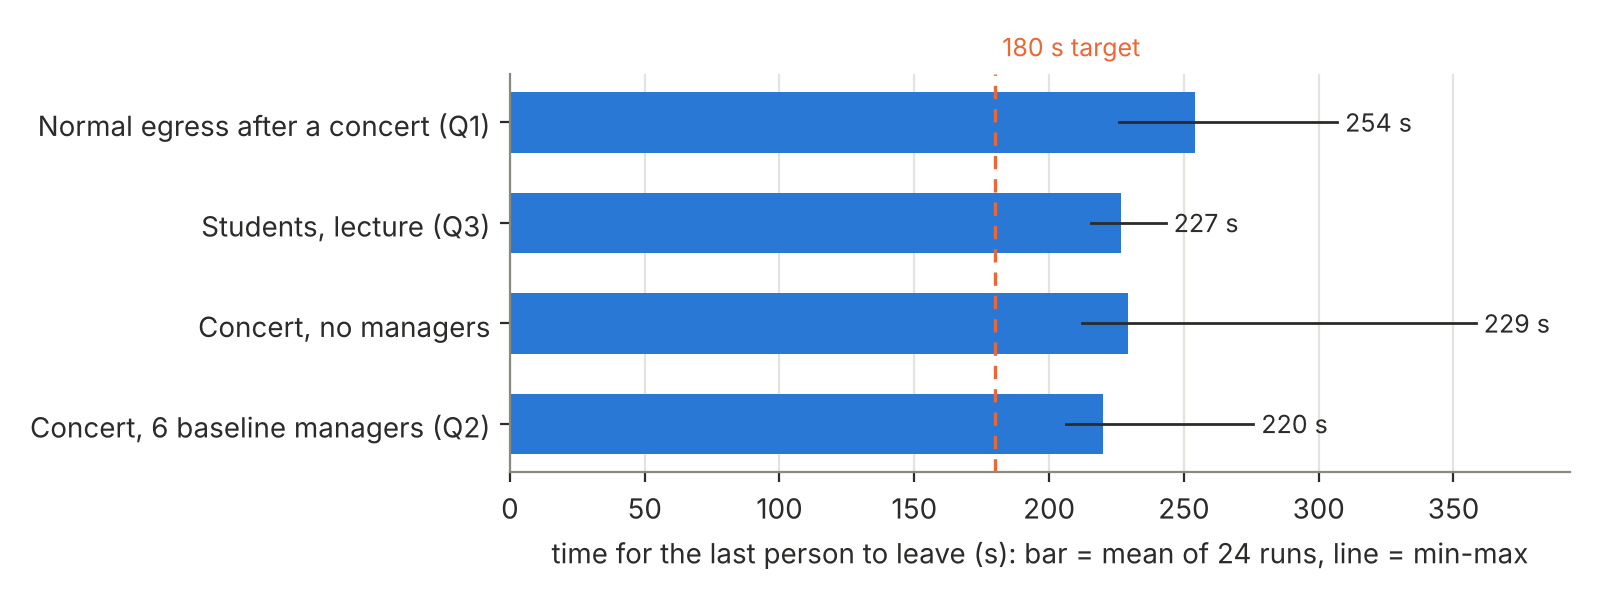
\includegraphics[width=0.9\linewidth]{fig/fig_scenarios.png}
    \caption{Mean time for the last person to leave in each scenario (bars) and the range over 24 runs (lines). The dashed line is the 180\,s target.}
    \label{fig:scenarios}
\end{figure}

\begin{table}[H]
    \centering
    \small
    \begin{tabular}{lccccccc}
        \toprule
        & \multicolumn{2}{c}{Students} & \multicolumn{2}{c}{Concert, no managers} & \multicolumn{2}{c}{Concert, baseline managers}\\
        Exit & People & Clears (s) & People & Clears (s) & People & Clears (s) \\
        \midrule
        F1--F5 (front doors) & 230 & 130 & 301 & 163 & 301 & 170 \\
        PW (west portico) & 385 & 226 & 425 & 225 & 416 & 215 \\
        PE (east portico) & 385 & 168 & 481 & 224 & 473 & 212 \\
        SW + SE (stage) & 181 & 122 & -- & -- & 18 & 85 \\
        BW + BE (balcony, stage side) & 148 & 110 & 122 & 101 & 122 & 102 \\
        \bottomrule
    \end{tabular}
    \caption{Mean number of people leaving through each exit, and the mean time at which the last of them leaves (including the stair time for BW/BE).}
    \label{tab:exits}
\end{table}

Three things stand out in Table~\ref{tab:scenarios} and Figure~\ref{fig:scenarios}. First, \textbf{no scenario meets the 180-second target in any run.} Second, the spread between runs is usually small (a standard deviation of about 5--15\,s), apart from rare runs in which the queue at a portico door jams: one unmanaged concert run of 24 took 358\,s, against a median of 222\,s. We therefore report medians alongside means. Third, Table~\ref{tab:exits} shows where the time goes: in every scenario the two portico doors are the last exits to clear. Each is a single 4\,ft door, yet each carries 300--400 people because it is by far the nearest exit for anyone leaving the loge by a side door. The five front doors and the stage-side routes are finished well before the portico doors.

\textbf{Queues, more than reaction, set the time.} With the response-time distribution of \cite{galea2017}, the median person is not ready to move until 51\,s after the alarm. Yet in an earlier version of our model in which everyone moved at once, the unmanaged concert evacuation still took 213\,s, only about 16\,s less than with response times. Most people are ready long before their turn at a portico door comes, so it is the queue at the portico doors, not the reaction of the audience, that determines when the last person leaves. Measures that rebalance the load between exits therefore have more to offer than measures that make people react faster, although both help.

\subsection{Q1: Normal egress after a concert}
After a concert there is no alarm and no reason to use unfamiliar doors, so the audience leaves the way it came in: through the vestibule, the foyer and the five front doors, and down the two main balcony staircases. We assume everyone is ready to leave within 30\,s of the end of the show. The house then empties in 254\,s on average (226--307\,s), with 90\% out after 176\,s. This is slower than the emergency evacuation even though people start sooner, because the whole audience is funnelled through the three 5\,ft doors between the vestibule and the foyer: about 1,300 people through 4.6\,m of doorway. For ordinary departures this is acceptable, and opening the portico doors at the end of large events would be the simplest way to speed them up.

\subsection{Q2: Concert evacuation with Crowd Managers}
With six Crowd Managers at the baseline posts of Table~\ref{tab:baseline_posts}, the concert audience is out in 220\,s on average (206--276\,s), compared with 229\,s with no managers at all. The managers spoke to about 564 people in each run. Their effect is modest because the baseline posts mostly confirm what people would do anyway: the corridor managers send people to the portico doors, which those people had already chosen, and so they add to the queue at the bottleneck rather than relieving it. The two managers at the front of the orchestra add the stage escape routes, which the audience does not know about, but only for the people sitting near them.

\textbf{Unexpected obstructions.} Closing the two central front doors F2 and F3 without warning leaves the mean evacuation time essentially unchanged (219\,s versus 220\,s). The front doors are not the bottleneck: people discover the closure in the foyer, within a few metres of the three remaining front doors, and switch to F1, F4 or F5 at little cost. A closure of the west portico door PW is more serious: the mean rises to 236\,s. Here the managers' knowledge matters, since the corridor manager on the west side, who knows about the closure, sends people to the west stage escape route instead; about 265 people leave that way. In both cases the plan degrades gracefully rather than collapsing, which is the property we want from a plan that confused people must execute.

\subsection{Q3: Students in a lecture}
Students who know every exit evacuate in 227\,s on average (216--243\,s). Perhaps surprisingly, this is no faster than the unmanaged concert audience (229\,s, median 222\,s) and slower than the concert audience with Crowd Managers (220\,s). Students do use the stage escape routes and the stage-side balcony stairs from the start, sending about 75 and 106 people through SW and SE, which the concert audience does not know about. But knowledge alone does not solve the problem: because every student independently picks the exit nearest to them, 385 of them converge on the west portico door and 385 on the east, and the last student leaves through PW at about 226\,s while the front doors are finished at about 130\,s. This is the situation the problem statement warns about: what is best for each individual impedes the group. Closing F2 and F3 barely affects students (229\,s), since they simply use the other front doors.

\subsection{Q4: Optimizing Crowd Manager posts}
\label{sec:opt_managers}
The greedy search of Section~\ref{sec:design} was run with an earlier version of our model in which everyone was ready to move at the moment of the alarm (no response-time delay) and LED strips acted through a fixed follow probability. The absolute times below are therefore not directly comparable with Table~\ref{tab:scenarios} (the unmanaged concert took 213\,s in that version against 229\,s now). We report them for the \emph{relative} value of each measure, which is what the search optimizes.

\begin{table}[H]
    \centering
    \small
    \begin{tabular}{clccc}
        \toprule
        Managers & Post added (location $\to$ exit) & Mean $T_{100}$ (s) & 95\% CI & Mean $T_{90}$ (s)\\
        \midrule
        0 & -- & 212.8 & $\pm$2.1 & 156.7 \\
        1 & side corridor W $\to$ PW & 209.0 & $\pm$2.9 & 153.7\\
        2 & mid cross aisle E $\to$ PE & 204.4 & $\pm$2.0 & 150.4\\
        3 & mid cross aisle W $\to$ PW & 198.4 & $\pm$2.3 & 148.5\\
        4 & side corridor E $\to$ PE & 199.1 & $\pm$3.2 & 147.7\\
        5 & balcony SE $\to$ PW & 196.5 & $\pm$3.2 & 146.6\\
        6 & rear ring W $\to$ PW & 198.7 & $\pm$3.2 & 147.1\\
        \midrule
        7 & balcony SW $\to$ PW & 198.6 & $\pm$2.6 & 146.3\\
        8 & foyer $\to$ F3 & 200.1 & $\pm$4.5 & 147.5\\
        \bottomrule
    \end{tabular}
    \caption{Greedy Crowd Manager search (earlier model version without response delay; 24 seeds per row). Each row adds the post that most reduced the mean evacuation time.}
    \label{tab:greedy_managers}
\end{table}

\begin{figure}[H]
    \centering
    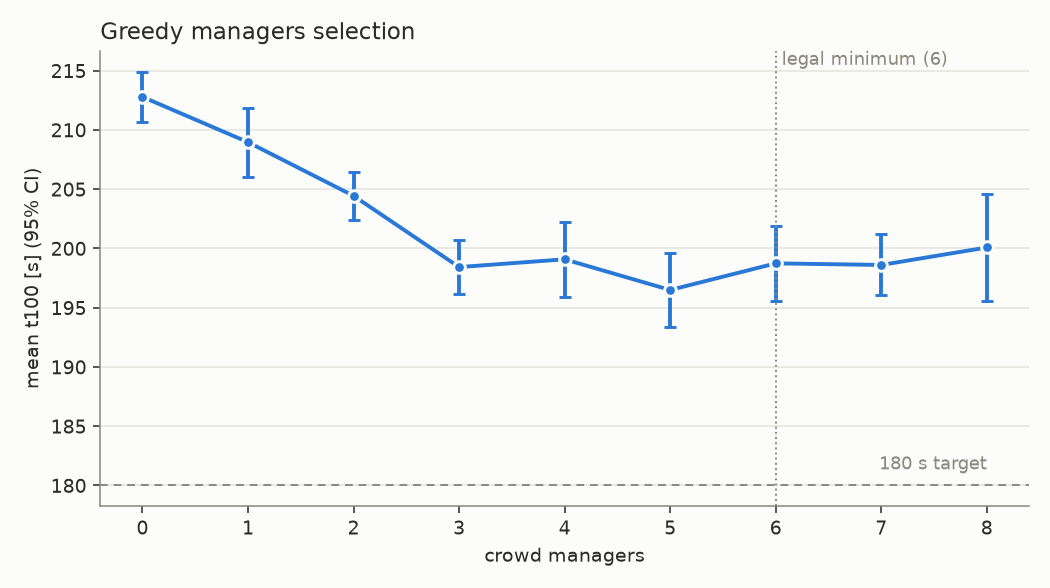
\includegraphics[width=0.49\linewidth]{fig/managers_curve.png}
    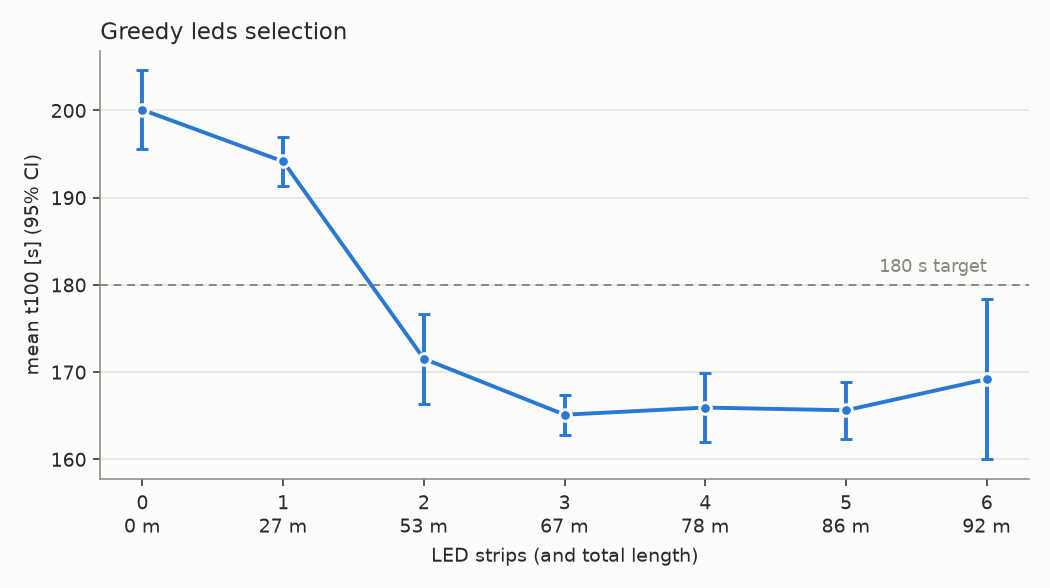
\includegraphics[width=0.49\linewidth]{fig/leds_curve.png}
    \caption{Mean evacuation time as managers (left) and LED strips (right) are added by the greedy search, with 95\% confidence intervals (earlier model version).}
    \label{fig:curves}
\end{figure}

The search (Table~\ref{tab:greedy_managers}, Figure~\ref{fig:curves}, left) cuts the evacuation time by about 14\,s, or 7\%, with six well-placed managers, compared with no managers at all. Almost all of the gain comes from the first three. Managers beyond the sixth bring nothing measurable: the seventh and eighth leave the mean within its confidence interval. The best posts are in the mid cross aisles and the side corridors on the first floor, where the side-door streams form, and at the south ends of the balcony.

The search never reaches 180\,s, even with no response delay at all, and its choices reveal why. Every post it picks sends people to a portico door or to the front doors; it never picks a post that diverts people \emph{away} from the portico doors toward the stage escape routes, because a manager can only redirect people who pass within 4\,m, and the side-door crowds are too large for one manager to talk to in time. Managers, in short, can choreograph the crowd near them, but they cannot rebalance a building-wide flow on their own. That is the job for the environmental measures.

\subsection{Q4a: Temporary barriers in the corridor}
The portico barriers of Section~\ref{sec:barriers} split the corridor into a portico zone and a foyer zone. Their effect depends strongly on who is in the hall (Table~\ref{tab:scenarios}). For the unmanaged concert audience they reduce the mean evacuation time from 229\,s to 224\,s. With the baseline managers the time is 219\,s against 220\,s without barriers, and for students it is 239\,s against 227\,s.

For the concert audience the barriers barely change the \emph{typical} evacuation: the medians with and without barriers are within a few seconds of each other. What they change is the \emph{worst case}. Without barriers, the queue at a portico door occasionally jams where it crosses the stream of people walking along the corridor toward the foyer; the slowest of 24 runs took 358\,s unmanaged and 276\,s with managers. With the barriers, nobody walks past a portico queue on the way to somewhere else, and the slowest runs took only 234\,s and 234\,s; the standard deviation falls from 29\,s to 5\,s without managers. The barriers also move about 262 people per run from the portico doors to the front doors (Table~\ref{tab:barrier_exits}), which is the right direction, although not enough to change which exit clears last.

\begin{table}[H]
    \centering
    \small
    \begin{tabular}{lcccc}
        \toprule
        & \multicolumn{2}{c}{Concert, baseline managers} & \multicolumn{2}{c}{Students}\\
        & no barriers & barriers & no barriers & barriers\\
        \midrule
        People through PW + PE & 888 & 626 & 770 & 612\\
        People through F1--F5 & 301 & 564 & 230 & 388\\
        Last out at PW (s) & 215 & 214 & 226 & 239\\
        Slowest run (s) & 276 & 234 & 243 & 255\\
        \bottomrule
    \end{tabular}
    \caption{Effect of the portico barriers on exit use (mean over 24 runs).}
    \label{tab:barrier_exits}
\end{table}

For students the barriers make things worse, by about 12\,s. Students already spread themselves across the exits they know; the barriers take away their second route to each portico door (out through an aisle door and north along the corridor), so everyone bound for a portico door must now pass through the single side door of the loge, and the two doors in series form a tighter bottleneck than before. Barriers thus trade flexibility for predictability. That trade is worth making for an audience that does not know the building and benefits from having fewer, clearer choices, and not worth making for one that does. Since the barriers are temporary, the practical conclusion is to set them up for concerts and leave them out for lectures.

\begin{figure}[H]
    \centering
    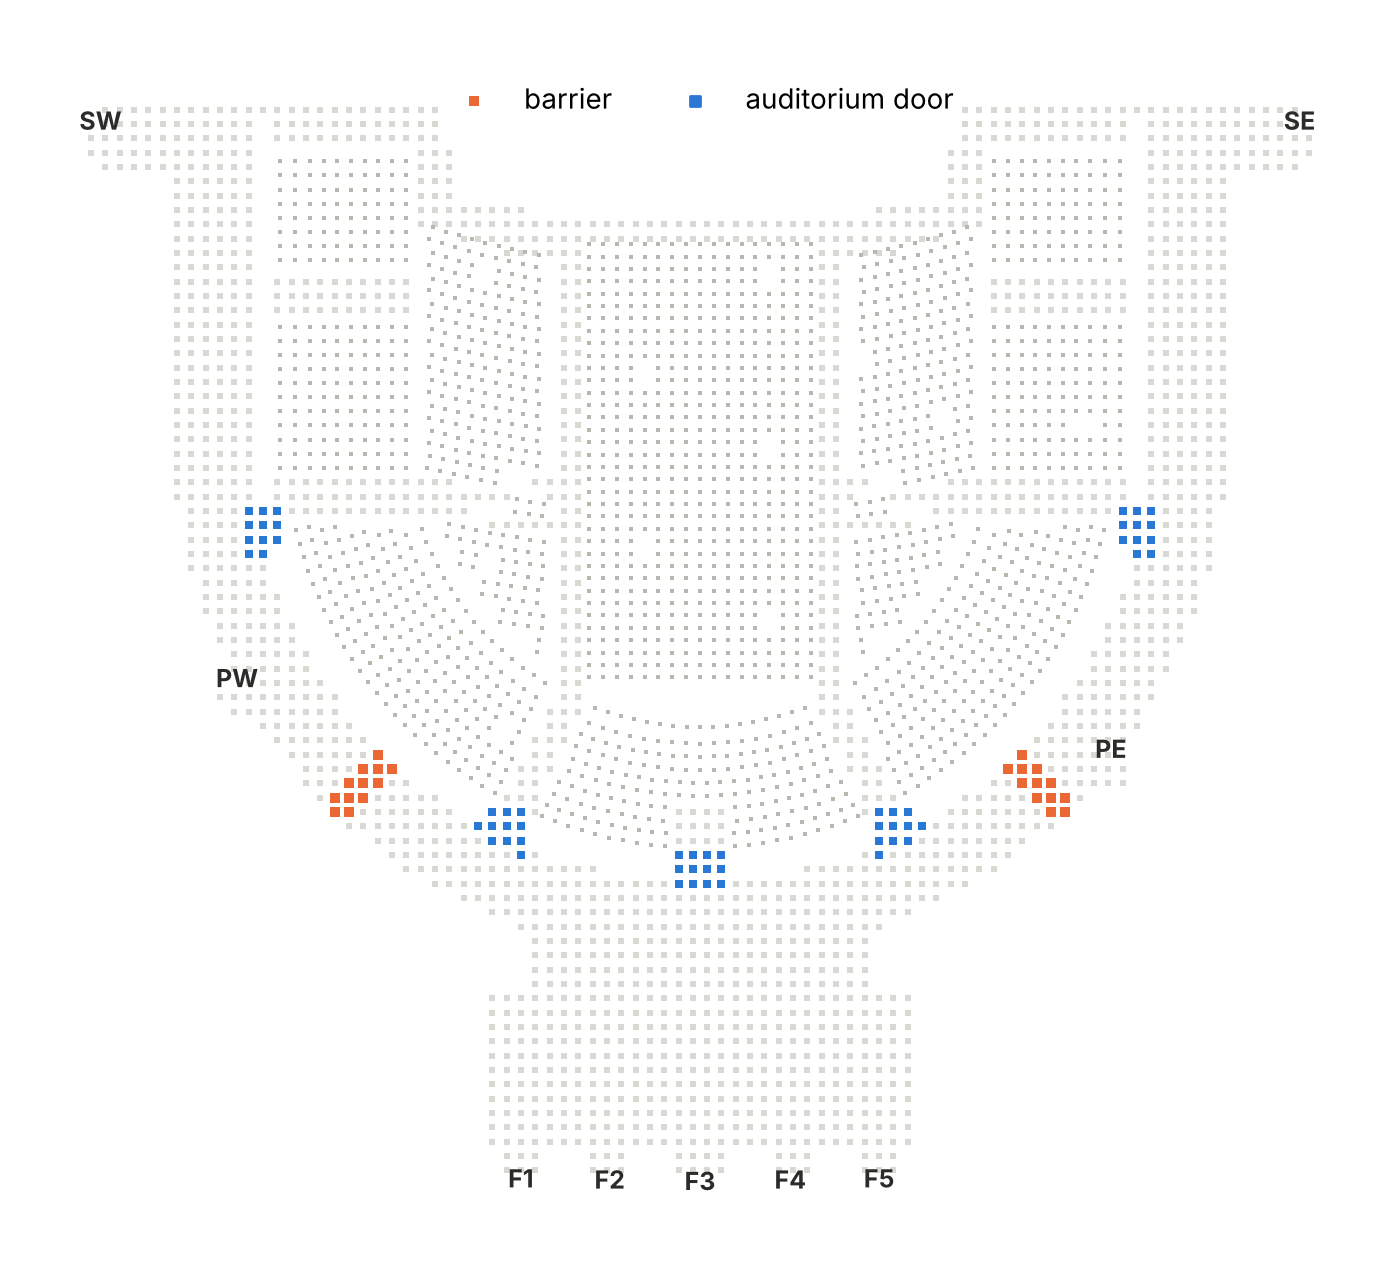
\includegraphics[width=0.6\linewidth]{fig/fig_barriers.png}
    \caption{The portico barriers (orange) on the first floor. Each closes the corridor between a portico door and the vestibule, so the loge side doors feed the portico doors and the aisle and centre doors feed the foyer.}
    \label{fig:barriers}
\end{figure}

\subsection{Q4b: LED strips}
We ran the greedy LED search with the eight managers of Table~\ref{tab:greedy_managers} fixed in place (earlier model version). Since the seventh and eighth managers changed the mean by less than 2\,s, well within the confidence interval, we expect the LED results to carry over to six managers.

\begin{table}[H]
    \centering
    \small
    \begin{tabular}{clccc}
        \toprule
        Strips & Strip added (start $\to$ exit) & Total length (m) & Mean $T_{100}$ (s) & 95\% CI\\
        \midrule
        0 & -- & 0 & 200.1 & $\pm$4.5\\
        1 & centre aisle W $\to$ F2 & 26.7 & 194.2 & $\pm$2.8\\
        2 & centre aisle E $\to$ F4 & 53.3 & 171.5 & $\pm$5.2\\
        3 & mid cross aisle E $\to$ PE & 66.8 & 165.1 & $\pm$2.3\\
        4 & mid cross aisle W $\to$ PW & 77.7 & 165.9 & $\pm$4.0\\
        5 & loge back centre $\to$ F3 & 86.2 & 165.6 & $\pm$3.2\\
        6 & rear ring W $\to$ PW & 91.9 & 169.2 & $\pm$9.2\\
        \bottomrule
    \end{tabular}
    \caption{Greedy LED strip search with the managers fixed (earlier model version; 24 seeds per row).}
    \label{tab:greedy_leds}
\end{table}

\begin{figure}[H]
    \centering
    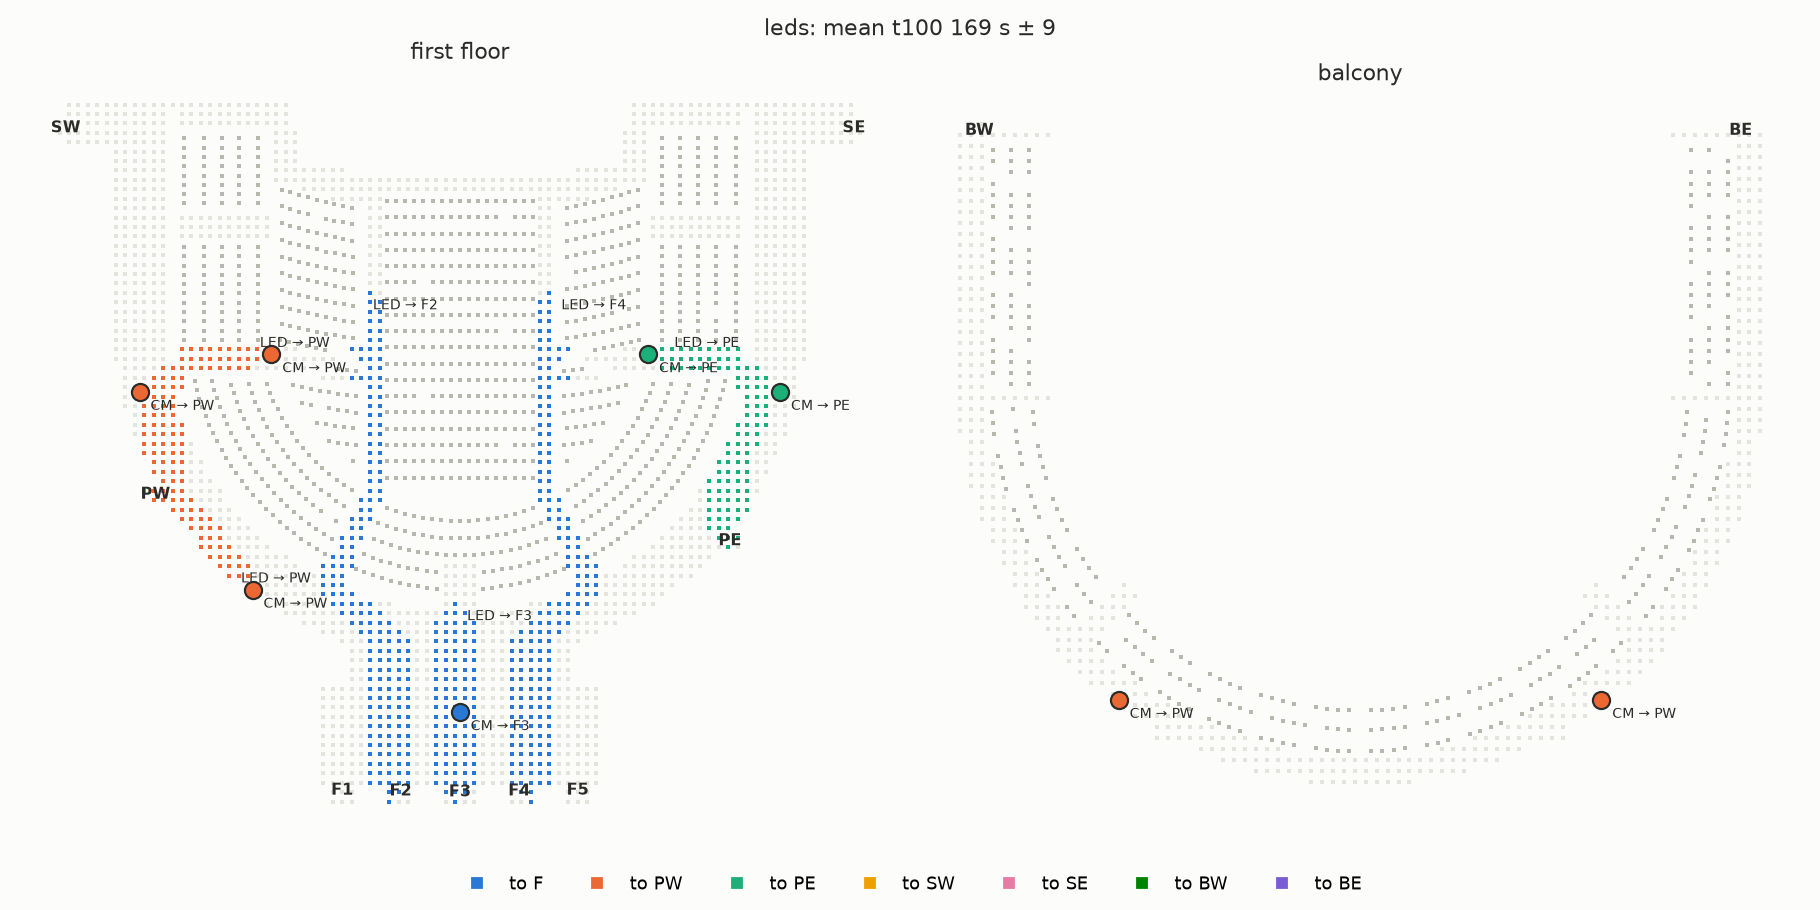
\includegraphics[width=\linewidth]{fig/leds_layout.png}
    \caption{The managers (circles) and the six LED strips chosen by the search, coloured by the exit they lead to.}
    \label{fig:led_layout}
\end{figure}

LED strips are by far the most effective measure we tested. The first two strips, running up the two centre aisles of the orchestra and on through the aisle doors and the vestibule to the front doors F2 and F4, cut the mean evacuation time by about 29\,s (14\%), twice what all six managers achieved. A third strip, from the east mid cross aisle to PE, brings the total saving to 35\,s (17\%), with 67\,m of strip. The strips beyond the third add nothing. The reason is the same bottleneck: the two centre-aisle strips draw the orchestra away from the side doors, and therefore away from the overloaded portico doors, toward the five front doors, which have spare capacity. In the runs with these strips, use of the west portico door falls from about 573 to about 412 people and use of the front doors rises by about 70\%, from 288 to 493 people. In other words, the strips do the building-wide rebalancing that managers cannot, and they do it without the panic-prone step of reversing anyone's direction: people simply drift toward the strip that is in front of them.

Because the LED strips act on routing, and routing is what limits the evacuation, we expect their absolute saving to carry over to the full model. In the earlier version, optimized managers plus the first three strips took the unmanaged time of 213\,s down to 165\,s, a saving of about 48\,s. Subtracting the same saving from the current unmanaged time gives roughly 180\,s for the full model: at the target, but not reliably below it. This is an estimate, not a simulation result, and confirming it with the full model is the first item of future work.

\textbf{LEDs and obstructions.} The strips do not know about closures (Section~\ref{sec:obstructions}). The two most useful strips lead to F2 and F4, so a closure of one of those doors would send part of the audience into a dead end until they come within 4\,m of it, after which their trust in the strips falls. Since the front doors are adjacent and the foyer is open, the cost of such a detour is small; but an LED installation should be wired to the fire alarm panel so that strips leading to a door reported blocked can be switched off. A dark strip is far better than one pointing the wrong way.

\subsection{Q5: Cost-effectiveness}
\textbf{Crowd Managers.} The median wage of a security guard in the United States is \$18.28 per hour \cite{bls2025}. Adding 30\% for payroll taxes, training and supervision, and assuming a four-hour shift per event, an additional Crowd Manager costs about \$95 per event. For a venue that hosts, say, 50 large non-academic events a year, that is about \$4,750 per manager per year, recurring.

\textbf{LED strips.} Installed LED strip lighting costs \$8--\$18 per foot, plus \$40--\$150 per power supply and \$35--\$120 per controller, and possibly \$50--\$150 in permits \cite{countbricks2026}. The two centre-aisle strips (53\,m, or 175\,ft) would cost about \$1,400--\$3,150 in strip and installation, plus perhaps \$500 for power supplies and a controller, so roughly \$2,000--\$3,700. Egress path marking must keep working when the main power fails, which requires battery backup or a photoluminescent backing; doubling the estimate to allow for this gives \$4,000--\$7,400. The full three-strip layout (67\,m, 220\,ft) would cost about 25\% more.

\textbf{Barriers.} The portico barriers need about 4\,m of stanchions and belt on each side. At a few hundred dollars per post, the pair costs under \$1,500, and they are reusable.

\textbf{Comparison.} The LED installation costs about as much as one extra Crowd Manager for 40--80 events, which at 50 large events a year is one to two seasons. But the comparison is not close in effect: in our simulations a seventh and eighth manager reduced the evacuation time by nothing measurable, while the first two LED strips reduced it by about 29\,s. LEDs are therefore by far the more cost-effective way to speed up the evacuation; extra managers are only worth paying for if they are placed where the six required managers are not, and the search found no such place.

\subsection{Sensitivity analysis}
Our results depend on several behavioral parameters that we could not calibrate directly against Bailey Hall. The most important is the response time: the first people are ready to move after 10--20\,s and the median person only after almost a minute, so any error in the response-time distribution of \cite{galea2017} shifts all our evacuation times by a similar amount. As noted above, removing the response delay entirely shortened the unmanaged evacuation by only about 16\,s in the earlier model version, because the portico queues dominate; but any error in the distribution still shifts our times. We therefore emphasize differences between scenarios, which are computed with identical response times (common random numbers), over absolute times.

The door capacities are the other main sensitivity. The 0.5\,m lattice lets about two people abreast through a 4\,ft portico door; in our runs, about 425 people pass through PW in about 225\,s, at least 1.9 people per second. Engineering guidance gives a maximum specific flow of about 1.3 people per second per metre of effective width \cite{sfpe2016}, or about 1.2 people per second for this door. Our portico doors are thus optimistic, perhaps by as much as half, so the real queues there could be longer than we predict. This strengthens our conclusion that they are the bottleneck, and means our absolute times are, if anything, too short.

Finally, the stochasticity of the model is small relative to the effects we report: the standard deviation of $T_{100}$ across seeds is 5--15\,s in every scenario, and differences between configurations measured on common seeds are more precise still.

\section{Strengths and Weaknesses}
\subsection{Strengths}
\begin{itemize}
    \item \textbf{Faithful geometry.} The building is modelled to scale from the official plans, with every seat in its real position, both levels, the barrier between orchestra and loge, the staircases and all eleven exits. The bottleneck we identify is a property of the real floor plan, not of a schematic.
    \item \textbf{Behavior grounded in data.} Response times follow a published study of a theatre audience \cite{galea2017}, including their dependence on seat position and the social cue of a neighbor standing up. Walking speeds follow the pedestrian literature.
    \item \textbf{Knowledge is modelled explicitly.} The concert audience and the students differ in what they know, closures are discovered locally, and managers and LEDs act on information rather than on movement. This lets us ask the questions posed: what managers add, and what happens when an exit is unexpectedly blocked.
    \item \textbf{Reproducible comparisons.} Every configuration is evaluated on the same random seeds, so comparisons between them are much more precise than the run-to-run spread, and the optimization is reproducible.
\end{itemize}

\subsection{Weaknesses}
\begin{itemize}
    \item \textbf{The optimization used an earlier model version.} The manager and LED searches were run before response times were added to the model. Their relative conclusions are consistent with the full model's diagnosis (the portico doors are the bottleneck), but their absolute times are not directly comparable, and the searches should be repeated with the full model.
    \item \textbf{Crowd Managers only redirect.} Real managers also announce the evacuation, prompting people to stand up sooner, and hold doors open. Crediting them with shorter response times would likely be the single largest improvement, but we had no data to calibrate it.
    \item \textbf{Response times dominate.} Since the median person waits about 51\,s before moving, our absolute times are sensitive to a distribution measured in a different theatre.
    \item \textbf{Simplified physics.} A cellular automaton has no pushing, no counter-flow negotiation and no body contact. People cannot pass one another in a one-cell-wide space, and stairs are modelled only as slower floor.
    \item \textbf{No groups and no special needs.} Families do not wait for each other, and wheelchair users and others needing assistance are represented only by slow walking speeds.
    \item \textbf{Grid effects at narrow doors.} On a 0.5\,m grid, a 4\,ft door is two or three cells wide depending on where it falls; the west portico door is one cell narrower than the east, which is one reason PW is usually the last exit to clear. The door flows are also higher than engineering guidance (see the sensitivity analysis).
    \item \textbf{Hand-picked candidates.} The search covers 33 manager posts and 33 LED strips chosen by hand. A different candidate set might do better, and greedy search is not guaranteed to find the best combination.
\end{itemize}

\section{Conclusion}
We built a to-scale agent-based model of Bailey Hall and used it to estimate how long the hall takes to empty in an ordinary departure, in an emergency with and without Crowd Managers, and in a lecture, and to evaluate barriers, LED strips and the placement of Crowd Managers.

The answer to the Fire Marshal's central question is sobering but clear. With the reaction times observed in a real theatre audience and the building as it is, none of our scenarios empties the hall within 180 seconds: a managed concert audience takes about 220\,s, students about 227\,s, and an ordinary departure about 254\,s. The binding constraint is not the front doors, which are robust even to an unexpected closure, but the two narrow portico doors, which take more than half of the audience. Everyone acting rationally on their own sends too many people there; this is why informed students are no faster than an uninformed concert audience.

Crowd Managers help, and six well-placed managers are better than six placed by intuition; but a seventh or eighth adds nothing, because managers can only influence the people near them. Temporary barriers in the corridor make the concert evacuation more predictable without making it faster, and should not be used for lectures. Directional LED strips are the most effective and the most cost-effective measure: two strips up the centre aisles of the orchestra draw people away from the portico doors toward the front doors, saving about 30\,s for roughly the cost of one extra Crowd Manager over a season or two. Our best estimate is that optimized managers and LED strips together would bring a managed concert evacuation close to the 180-second target, though not reliably below it.

Good evacuation guidance has to survive being executed by frightened people. The measures we recommend share that property: a strip of light that says ``this way'', a barrier that removes a wrong choice, and a manager who repeats one instruction. Their legibility, more than their cleverness, is what we expect to make them work.

\textbf{Future work.} The first priority is to repeat the manager and LED searches with the full model, including response times, and to evaluate the LED strips under exit closures. Beyond that, we would credit Crowd Managers with shortening reaction times by announcing the evacuation, calibrate door flows against engineering data, and test other barrier layouts, such as ones that route the side-door streams to the stage escape routes.

\begin{thebibliography}{99}

\bibitem{nist2010}
Kuligowski, E. D., Peacock, R. D., and Hoskins, B. L.
\textit{A Review of Building Evacuation Models},
2nd ed., NIST Technical Note 1680, 2010.

\bibitem{galea2017}
Galea, E. R., Deere, S. J., Hopkin, C. G., and Xie, H.
\textit{Evacuation Response Behaviour of Occupants in
a Large Theatre during a Live Performance}, 2017.

\bibitem{simeHUMANBEHAVIOURFIRES}
Sime, J. D. (n.d.). \textit{Human Behaviour in Fires -- Summary Report}.

\bibitem{burstedde2001}
Burstedde, C., Klauck, K., Schadschneider, A., and Zittartz, J.
\textit{Simulation of Pedestrian Dynamics Using a Two-Dimensional Cellular Automaton}.
Physica A, 295(3--4), 507--525, 2001.
https://doi.org/10.1016/S0378-4371(01)00141-8

\bibitem{kirchner2002}
Kirchner, A., and Schadschneider, A.
\textit{Simulation of Evacuation Processes Using a Bionics-Inspired Cellular Automaton Model for Pedestrian Dynamics}.
Physica A, 312(1--2), 260--276, 2002.
https://doi.org/10.1016/S0378-4371(02)00857-9

\bibitem{bls2025}
U.S. Bureau of Labor Statistics, via O*NET OnLine,
``Local Wages: Security Guards (33-9032.00),''
May 2025 data.
\url{https://www.onetonline.org/link/localwages/33-9032.00}.

\bibitem{countbricks2026}
CountBricks,
``Trim Lighting Costs for Construction Professionals,''
2025.
\url{https://www.countbricks.com/post/how-much-does-trim-lighting-cost}.

\bibitem{sfpe2016}
Gwynne, S. M. V., and Rosenbaum, E. R.,
``Employing the Hydraulic Model in Assessing Emergency Movement,''
in \emph{SFPE Handbook of Fire Protection Engineering}, 5th ed., Springer, 2016.

\bibitem{weidmann1993}
U.~Weidmann,
\emph{Transporttechnik der Fussg\"anger: Transporttechnische Eigenschaften
des Fussg\"angerverkehrs (Literaturauswertung)},
Schriftenreihe des IVT Nr.~90, 2nd ed., ETH Z\"urich, March 1993.

\bibitem{helbing1995}
D.~Helbing and P.~Moln\'ar,
Social force model for pedestrian dynamics,
\emph{Physical Review E} \textbf{51}(5), 4282--4286, 1995.
doi:10.1103/PhysRevE.51.4282.

\bibitem{daamen2007}
W.~Daamen and S.~P.~Hoogendoorn,
Free speed distributions --- based on empirical data in different traffic
conditions,
in \emph{Pedestrian and Evacuation Dynamics 2005}, Springer, 2007.
doi:10.1007/978-3-540-47064-9\_2.

\bibitem{bohannon1997}
R.~W.~Bohannon,
Comfortable and maximum walking speed of adults aged 20--79 years:
reference values and determinants,
\emph{Age and Ageing} \textbf{26}(1), 15--19, 1997.
doi:10.1093/ageing/26.1.15.

\end{thebibliography}
\end{document}
